% !TEX root = ../main.tex

\section{实验结果与分析}

\subsection{模型站内分类性能}

% 数据：results/summary/within_site_crop_f1.csv（汇总口径）、within_site_crop_f1_fold_stats.csv（折间 std）
% 数字核对 2026-09-19：范围、最大差值、折间 std 均与 csv 一致

如图\ref{fig:within_site_f1}所示，三种模型在四个站点的站内玉米F1为90.98\%～96.23\%，大豆F1为89.55\%～95.89\%。三种模型表现出两点共性：一是在同一站点，玉米F1均高于大豆F1，差值为0.09～1.88个百分点；二是在不同站点之间，玉米和大豆F1均在A站点达到各自最高值。五折交叉验证中，12组实验（3种模型×4个站点）的玉米F1折间标准差为0.12～0.73个百分点，大豆F1为0.06～0.96个百分点，表明各模型的站内作物分类表现稳定。

\par\addvspace{3pt}
\noindent\begin{minipage}{\linewidth}
\captionsetup{type=figure}
\centering
\begin{subfigure}{\linewidth}
\centering
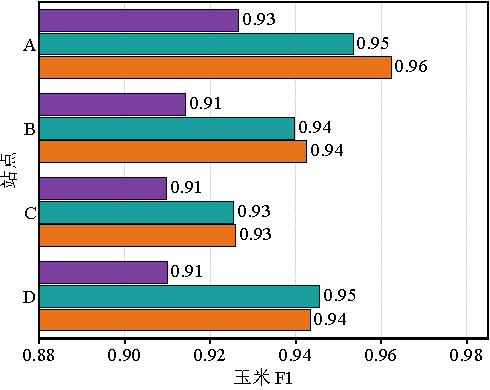
\includegraphics{results/fig_within_site_f1_a.pdf}
\caption{四站点玉米分类精度}
\end{subfigure}\par\nointerlineskip\vspace{3pt}
\begin{subfigure}{\linewidth}
\centering
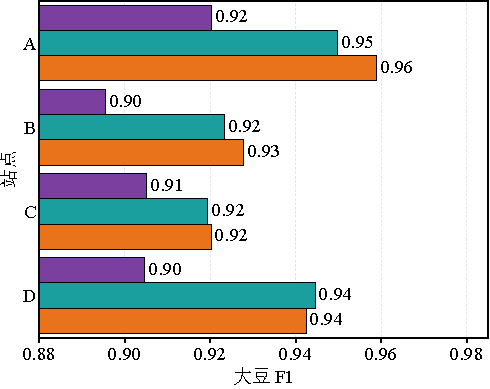
\includegraphics{results/fig_within_site_f1_b.pdf}
\caption{四站点大豆分类精度}
\end{subfigure}\par\nointerlineskip\vspace{3pt}
\modellegend
\caption{三种模型在四个站点的站内玉米和大豆分类精度}
\label{fig:within_site_f1}
\end{minipage}\par\addvspace{3pt}

三种模型之间存在较为稳定的精度差异。U-TAE和3D U-Net在各站点的玉米和大豆F1均高于ConvGRU，而U-TAE与3D U-Net之间的差值不超过1个百分点，二者互有高低：U-TAE在A、B、C三个站点略优，3D U-Net在D站点略优。ConvGRU的劣势幅度因站点而异：在C站点，三种模型的玉米和大豆F1最大差值分别为1.61和1.50个百分点；在D站点，该差值分别扩大至3.58和3.98个百分点。图\ref{fig:within_site_map_D}以D站点为例，直观对比了三种模型的站内交叉验证分类结果。以选中局部区域为例，ConvGRU的玉米和大豆像元错误率为12.1\%，明显高于3D U-Net（5.8\%）和U-TAE（4.8\%）。

% 图 3：上行全站 2560×2560 标红框，下行红框窗口放大；窗口 = D 站图块网格 (13,8) 起 2×2，像元行 1664–1920、列 1024–1280
% 选窗标准：只看真实玉米/大豆像元——作物像元错误率 ConvGRU 12.1% / 3D U-Net 5.8% / U-TAE 4.8%；
%   类别边界带错误率 32.0% / 15.3% / 13.4%；玉米↔大豆互混 6.8% / 2.6% / 2.2%。全站总错误率 10.6% / 6.3% / 6.7%
% 三模型 reference.tif sha256 一致（38ad33ef…）；oof_prediction.tif 为五折拼接，每图块预测来自未训练过它的模型

\begin{figure*}[tbp]
\centering
\begin{subfigure}{0.24\textwidth}\centering
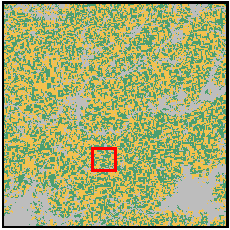
\includegraphics{results/fig_within_site_map_D_a.pdf}
\caption{参考标签}
\end{subfigure}\hfill
\begin{subfigure}{0.24\textwidth}\centering
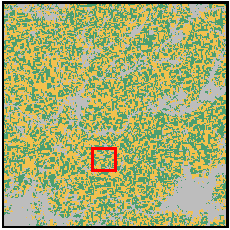
\includegraphics{results/fig_within_site_map_D_b.pdf}
\caption{ConvGRU分类结果}
\end{subfigure}\hfill
\begin{subfigure}{0.24\textwidth}\centering
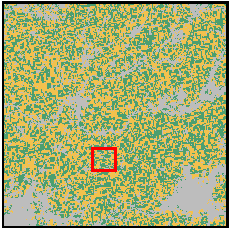
\includegraphics{results/fig_within_site_map_D_c.pdf}
\caption{3D U-Net分类结果}
\end{subfigure}\hfill
\begin{subfigure}{0.24\textwidth}\centering
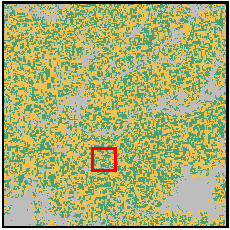
\includegraphics{results/fig_within_site_map_D_d.pdf}
\caption{U-TAE分类结果}
\end{subfigure}\par\nointerlineskip\vspace{3pt}
\begin{subfigure}{0.24\textwidth}\centering
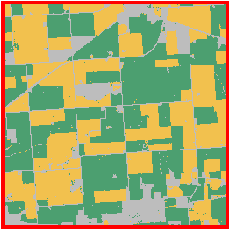
\includegraphics{results/fig_within_site_map_D_e.pdf}
\caption{参考标签}
\end{subfigure}\hfill
\begin{subfigure}{0.24\textwidth}\centering
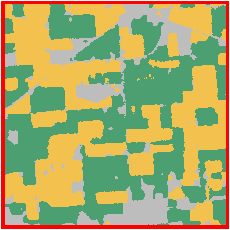
\includegraphics{results/fig_within_site_map_D_f.pdf}
\caption{ConvGRU分类结果}
\end{subfigure}\hfill
\begin{subfigure}{0.24\textwidth}\centering
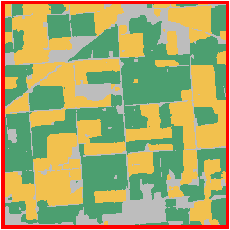
\includegraphics{results/fig_within_site_map_D_g.pdf}
\caption{3D U-Net分类结果}
\end{subfigure}\hfill
\begin{subfigure}{0.24\textwidth}\centering
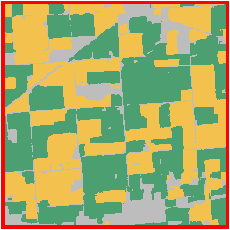
\includegraphics{results/fig_within_site_map_D_h.pdf}
\caption{U-TAE分类结果}
\end{subfigure}\par\nointerlineskip\vspace{3pt}
\classlegend
\caption{D站点三种模型站内交叉验证分类结果（上：全站，红框为局部窗口；下：局部窗口放大）}
\label{fig:within_site_map_D}
\end{figure*}

\FloatBarrier

\subsection{模型跨站分类性能与泛化退化}

% 数据：tables/table2_cross_site_f1_12paths.csv ← results/summary/cross_site_crop_f1_summary.csv（36 个模型—路径组合，5 次预测均值）
%       results/summary/within_site_crop_f1.csv（目标站站内汇总 F1，退化比例分母）
%       results/summary/crop_f1_relative_degradation_36paths.csv（图 4，泛化退化比例）
% 数字 2026-09-27 从上述文件现算；第一段范围取表内 36 格，最高值、最低值所在路径按模型逐一核对。

表\ref{tab:cross_site_f1_paths}给出了三种模型在12条迁移路径上的跨站玉米和大豆F1，每项为五次完整目标站预测的均值。源站模型不经微调直接用于目标站后，玉米F1为85.68\%～92.92\%，大豆F1为83.08\%～92.15\%，36个模型—路径组合的玉米和大豆F1均低于同一模型在目标站的站内汇总F1。按模型分别比较各条路径，三种模型的玉米和大豆跨站F1最高值均出现在以A站点为目标站的路径上，与站内结果中A站点精度最高相对应；三种模型的玉米跨站F1最低值则均出现在以C站点为目标站的路径上。

\begin{table*}[tbp]
\centering
\caption{三种模型在12条迁移路径上的跨站玉米和大豆F1}
\label{tab:cross_site_f1_paths}
{\songti\zihao{-5}
\renewcommand{\arraystretch}{1.12}
\setlength{\tabcolsep}{7pt}
\begin{tabular*}{\textwidth}{@{\extracolsep{\fill}}c*{6}{c}}
\toprule
\multirow{2}{*}{迁移路径} & \multicolumn{2}{c}{ConvGRU} & \multicolumn{2}{c}{3D U-Net} & \multicolumn{2}{c}{U-TAE} \\
\cmidrule(lr){2-3}\cmidrule(lr){4-5}\cmidrule(lr){6-7}
 & 玉米F1/\% & 大豆F1/\% & 玉米F1/\% & 大豆F1/\% & 玉米F1/\% & 大豆F1/\% \\
\midrule
A→B & 89.91 ± 0.11 & 87.52 ± 0.40 & 91.43 ± 0.39 & 89.28 ± 0.40 & 92.09 ± 0.26 & 89.90 ± 0.38 \\
A→C & 86.97 ± 0.59 & 86.94 ± 1.20 & 87.71 ± 0.59 & 87.96 ± 0.34 & 88.20 ± 0.61 & 88.29 ± 0.69 \\
A→D & 88.54 ± 0.67 & 88.05 ± 1.16 & 90.64 ± 0.53 & 90.56 ± 0.45 & 91.78 ± 0.43 & 91.48 ± 0.41 \\
B→A & 92.00 ± 0.18 & 91.59 ± 0.13 & 92.92 ± 0.59 & 92.15 ± 0.44 & 92.70 ± 0.25 & 91.87 ± 0.31 \\
B→C & 85.68 ± 0.95 & 84.52 ± 1.63 & 88.09 ± 0.55 & 88.20 ± 0.81 & 87.70 ± 0.58 & 87.66 ± 0.84 \\
B→D & 85.73 ± 1.67 & 83.08 ± 2.70 & 90.87 ± 0.33 & 90.43 ± 0.41 & 89.59 ± 1.41 & 88.50 ± 2.20 \\
C→A & 90.31 ± 0.59 & 90.15 ± 0.49 & 92.09 ± 0.40 & 91.64 ± 0.43 & 91.52 ± 0.61 & 91.09 ± 0.39 \\
C→B & 87.47 ± 1.05 & 85.06 ± 0.96 & 90.23 ± 1.00 & 88.98 ± 0.88 & 90.33 ± 0.62 & 88.18 ± 0.52 \\
C→D & 89.77 ± 0.29 & 89.57 ± 0.08 & 90.77 ± 0.85 & 90.91 ± 0.17 & 90.98 ± 0.39 & 90.70 ± 0.48 \\
D→A & 91.05 ± 0.24 & 90.85 ± 0.52 & 91.36 ± 0.68 & 91.32 ± 0.68 & 91.45 ± 0.26 & 92.04 ± 0.37 \\
D→B & 89.44 ± 0.24 & 86.19 ± 0.46 & 88.13 ± 1.24 & 86.19 ± 1.91 & 90.45 ± 0.45 & 89.17 ± 0.98 \\
D→C & 87.85 ± 0.30 & 88.19 ± 0.54 & 87.88 ± 0.71 & 88.60 ± 0.83 & 87.83 ± 0.89 & 88.41 ± 0.84 \\
\midrule
平均 & 88.73 & 87.64 & 90.18 & 89.69 & 90.39 & 89.77 \\
\bottomrule

\end{tabular*}
\par\nointerlineskip\vspace{3pt}
\begin{minipage}{\textwidth}
\noindent 注：箭头左侧为源站，右侧为目标站。每格为源站5个折模型分别预测目标站全部400个图块所得F1的算术平均，未进行微调和模型集成；“平均”为12条迁移路径F1均值的算术平均。
\end{minipage}
}
\end{table*}

% 第二段：12 条路径平均跨站 F1（表末行）；平均泛化退化比例 = 12 条路径比例的算术平均。
% 两种排序分别对应实际精度与相对同一模型目标站当地训练基准的差距。

按12条路径取算术平均，ConvGRU的跨站玉米和大豆F1分别为88.73\%和87.64\%，均低于3D U-Net（90.18\%、89.69\%）和U-TAE（90.39\%、89.77\%）。但同样对12条路径的泛化退化比例取算术平均，ConvGRU的玉米和大豆退化比例分别为3.05\%和3.32\%，小于3D U-Net（4.18\%、4.01\%）和U-TAE（4.21\%、4.22\%）。跨站F1反映模型在目标站的实际分类精度，泛化退化比例则衡量其与同一模型在目标站的站内汇总F1之间的相对差距。因此，泛化退化比例较小不代表跨站绝对精度更高，评价模型的跨站表现需要同时考察这两个指标。

% 第三段：图 4 数据 results/summary/crop_f1_relative_degradation_36paths.csv。
% 固定目标站 D：ConvGRU 大豆 C→D 0.99%、B→D 8.17%。
% B↔D：ConvGRU 玉米、大豆均 B→D 较大，3D U-Net 均 D→B 较大；比较基于各路径五次预测均值。

如图\ref{fig:degradation_heatmap}所示，按每条路径五次预测的F1均值计算的泛化退化比例随源—目标组合变化，不同模型的变化也不一致。固定D站点为目标站，ConvGRU的大豆泛化退化比例在源站为C时为0.99\%，源站为B时为8.17\%。在B、D两个站点之间，ConvGRU的玉米和大豆泛化退化比例均为B→D方向较大，3D U-Net则均为D→B方向较大；以大豆为例，ConvGRU在B→D和D→B路径上分别为8.17\%和3.75\%，3D U-Net分别为4.26\%和6.65\%。这一方向差异描述的是该站点对的均值表现，不代表普遍的迁移规律。这些路径差异的空间解释，还需结合各站点的地物组成与景观结构。

\begin{figure*}[tbp]
\centering
\begin{subfigure}{\dimexpr(\textwidth-6pt)/3\relax}\centering
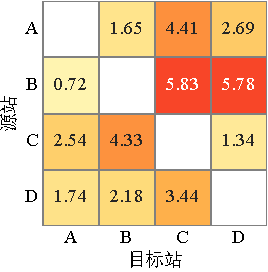
\includegraphics{results/fig_degradation_heatmap_a.pdf}
\caption{ConvGRU玉米泛化退化比例}
\end{subfigure}\hspace{3pt}%
\begin{subfigure}{\dimexpr(\textwidth-6pt)/3\relax}\centering
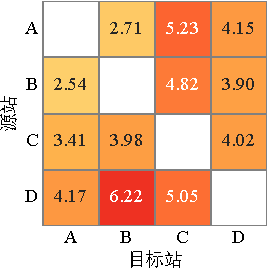
\includegraphics{results/fig_degradation_heatmap_b.pdf}
\caption{3D U-Net玉米泛化退化比例}
\end{subfigure}\hspace{3pt}%
\begin{subfigure}{\dimexpr(\textwidth-6pt)/3\relax}\centering
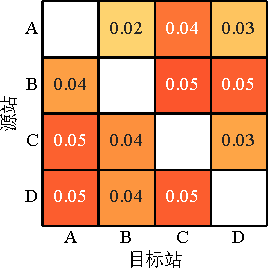
\includegraphics{results/fig_degradation_heatmap_c.pdf}
\caption{U-TAE玉米泛化退化比例}
\end{subfigure}\par\nointerlineskip\vspace{3pt}
\begin{subfigure}{\dimexpr(\textwidth-6pt)/3\relax}\centering
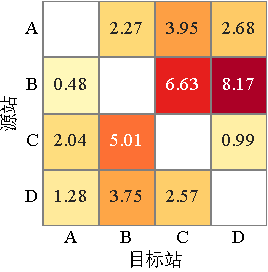
\includegraphics{results/fig_degradation_heatmap_d.pdf}
\caption{ConvGRU大豆泛化退化比例}
\end{subfigure}\hspace{3pt}%
\begin{subfigure}{\dimexpr(\textwidth-6pt)/3\relax}\centering
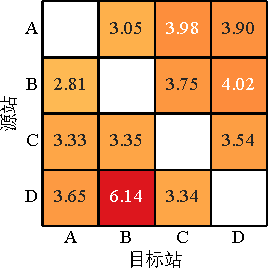
\includegraphics{results/fig_degradation_heatmap_e.pdf}
\caption{3D U-Net大豆泛化退化比例}
\end{subfigure}\hspace{3pt}%
\begin{subfigure}{\dimexpr(\textwidth-6pt)/3\relax}\centering
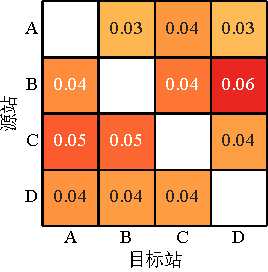
\includegraphics{results/fig_degradation_heatmap_f.pdf}
\caption{U-TAE大豆泛化退化比例}
\end{subfigure}\par\nointerlineskip\vspace{3pt}
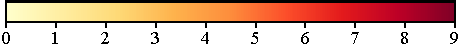
\includegraphics{results/fig_degradation_heatmap_cbar.pdf}\par\nointerlineskip\vspace{3pt}
{\songti\zihao{-5}泛化退化比例/\%\par}
\caption{不同源—目标区域组合下三种模型的玉米和大豆F1泛化退化比例（行为源站，列为目标站，对角线不适用）}
\label{fig:degradation_heatmap}
\end{figure*}

\FloatBarrier
\subsection{模型跨站泛化差异的空间解释}

% 数据（已生成，未入库）：图块级 D:/cross_site_all_20260916/paper_tables/Patch级空间误差底表/ 四张表；
%   站点级 D:/label/fragstats_results/完整标签{景观级,类别级}指标.csv（2023 年标签，ED 为景观级，AREA_MN、AI 为类别级）
% 方法：按空间特征分组后汇总混淆矩阵再算类别 F1；跨站逐次计算后再汇总 5 次结果，站内以同组图块为参照；不平均图块 F1
% 两个问题，覆盖全部站点与 12 条路径：目标站哪些空间条件下退化较大；同一目标站的退化随源站的变化与站点间哪些差异相对应
